\subsection{Digitale Ein- und Ausgabe: Hilfsschaltung} % (fold)
\label{sub:Digitale Ein- und Ausgabe: Hilfsschaltung}
    \begin{frame}
    \frametitle{Logikpegel}
    \framesubtitle{}
            \begin{figure}[H]
            \begin{center}
                    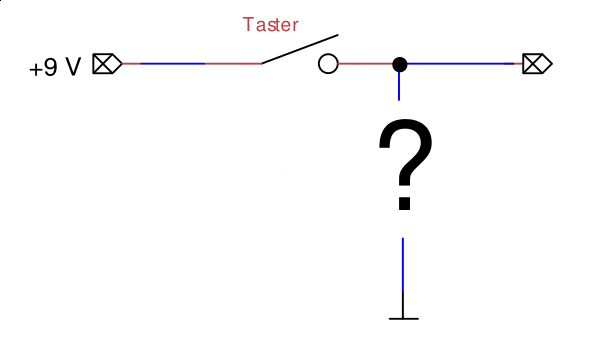
\includegraphics[scale=0.4]{./img/schaltung/logikpegel_1.png}
            \end{center}
            \end{figure}
    \end{frame}

\begin{frame}
    \frametitle{Logikpegel}
    \framesubtitle{}
    \begin{columns}[c]
        \column{0.6\textwidth}
        \begin{block}{}
                Pull-Down Widerstand von $R = 10k\Omega$ liefert High und Low:
        \end{block}
            \begin{center}
                \boxed{
                    \begin{tabular}{c|c}
                        H & $0.002V$ \\
                        L & $8.99V$
                    \end{tabular}
                }
            \end{center}
        \column{0.4\textwidth}
        \begin{figure}[H]
        \begin{center}
                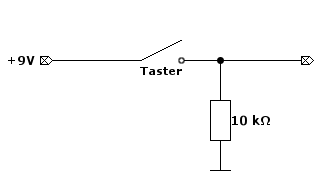
\includegraphics[scale=0.4]{./img/schaltung/logikpegel_2.png}
        \end{center}
        \end{figure}
    \end{columns}
\end{frame}

% subsection Digitale Ein- und Ausgabe: Hilfsschaltung (end)
